% Individual design study abstract -- Photonic Integrated Circuits, Aarhus University
% One PDF with title, abstract, schematic and selected references, as the
% design study guidelines ask. Compile with pdflatex (no bibliography run needed).
% references.bib holds the same references for the final report.

\documentclass[12pt,a4paper]{article}

\usepackage[utf8]{inputenc}
\usepackage[T1]{fontenc}
\usepackage{lmodern}
\usepackage[a4paper,margin=2.5cm]{geometry}
\usepackage{setspace}
\onehalfspacing
\usepackage{graphicx}
\usepackage{float}            % [H] keeps Figure 1 directly after the abstract
\usepackage{amsmath}
\usepackage[font=small,labelfont=bf]{caption}
\usepackage{siunitx}
\usepackage{microtype}
\usepackage{xcolor}
\usepackage[colorlinks=true, linkcolor=black, citecolor=black,
            urlcolor=blue!60!black]{hyperref}

\newcommand{\TE}[1]{TE$_{#1}$}
\newcommand{\TM}[1]{TM$_{#1}$}
\newcommand{\doi}[1]{\href{https://doi.org/#1}{doi:\,#1}}
\newcommand{\learned}{\textbf{What I learned.}\ }
\newcommand{\informs}{\textbf{How it informs my study.}\ }

\title{Access-Waveguide Width and the Fabrication Tolerance of
       Silicon Asymmetric Directional Couplers}
\author{Jacob Holm\\  % TODO: add surname / student number
        \small Photonic Integrated Circuits, Aarhus University\\
        \small Individual design study abstract}
\date{16 November 2026}

\begin{document}

\maketitle

% 245 words (limit 150-250). No citations and no results in the abstract.
\begin{abstract}
\noindent
Mode-division multiplexing raises link capacity by sending separate data channels
on different spatial modes of one waveguide. On silicon chips, the higher-order
modes are commonly excited by asymmetric directional couplers (ADCs), where each
narrow access waveguide's fundamental mode is phase-matched to a higher-order mode
of a wider bus. Because the two waveguides respond differently to a width error, a
few nanometers of deviation can break this condition. This design study asks
whether a narrower access waveguide gives a better balance between coupling
strength, phase matching and fabrication tolerance. Two couplers are studied,
\TE{0}--\TE{1} and \TE{0}--\TE{2}, on the standard \qty{220}{\nm}
silicon-on-insulator platform with oxide cladding at \qty{1550}{\nm}. The gap is
fixed at \qty{200}{\nm}, as in conventional designs, so any gain comes from the
access width alone. Narrowing the access waveguide strengthens the evanescent
coupling and shortens the coupler, but also increases the mismatch between the two
modes' width sensitivities. The hypothesis is that the stronger coupling outweighs
the larger mismatch, so tolerance improves until bend loss limits the access width.
Tolerance is defined as the largest uniform width error, applied to both waveguides
at fixed center spacing, for which the unconverted power stays below
\qty{-15}{\dB} at fixed coupler length. Effective indices, width sensitivities,
supermode splitting and bend loss are computed with the EMode2D mode solver and
combined through coupled-mode theory. The predictions are checked by mesh
convergence and against published coupler designs. The conclusions concern the
individual couplers, not a complete link.
\end{abstract}

\begin{figure}[H]
  \centering
  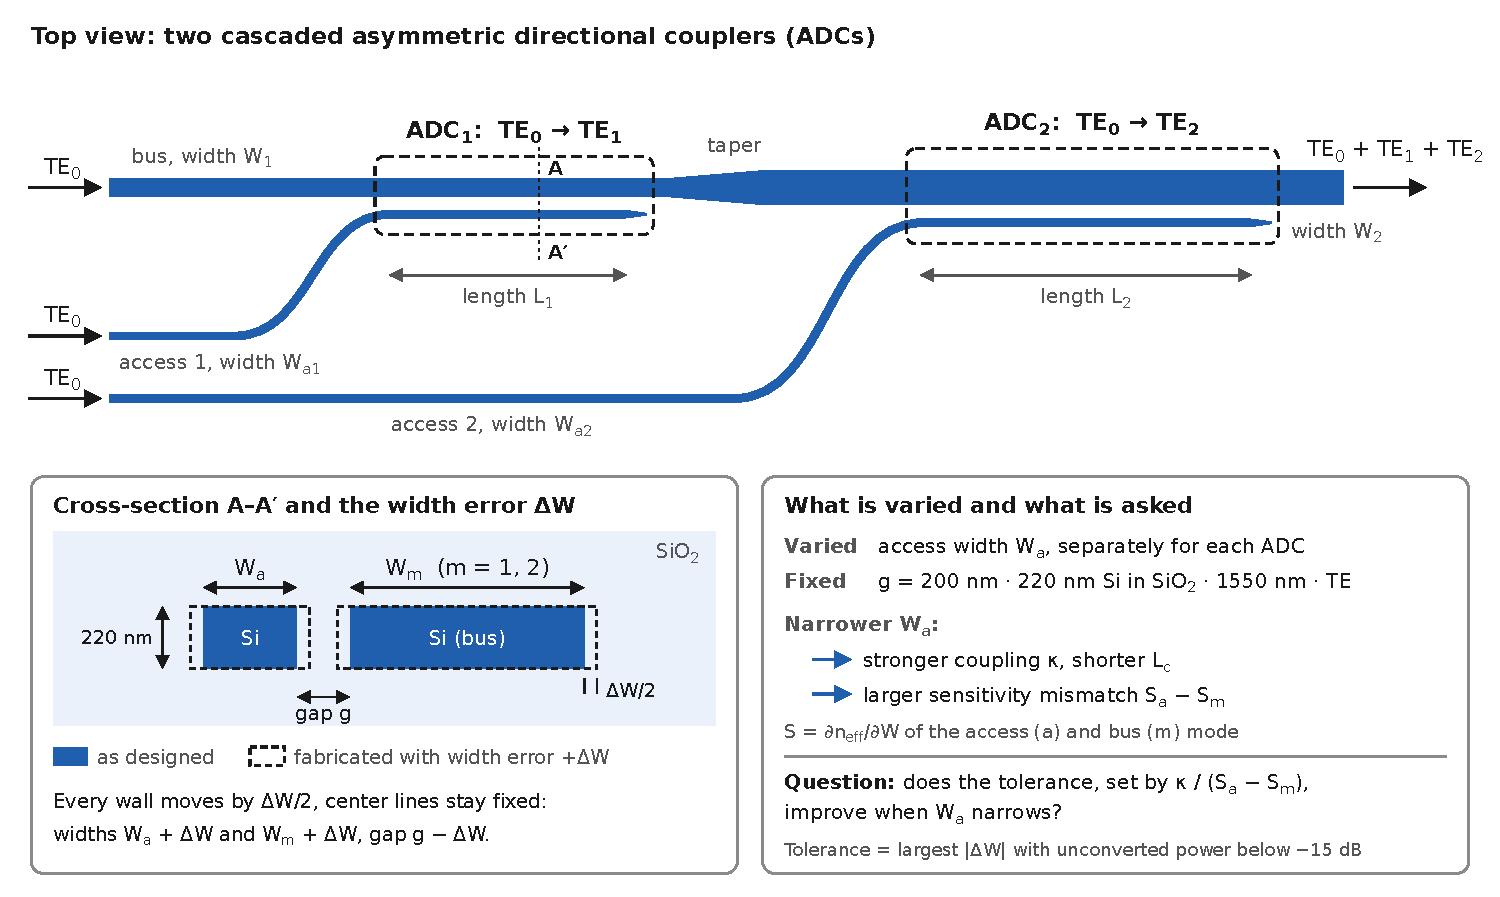
\includegraphics[width=\textwidth]{figures/adc_schematic.pdf}
  \caption{The two asymmetric directional couplers under study, in the cascaded
    layout of Dai et al.~[\ref{ref:dai}]. Top: each narrow access waveguide (widths
    $W_{a1}$, $W_{a2}$) runs beside the bus at gap $g$ over a length $L$ and
    converts its \TE{0} mode into the \TE{1} or \TE{2} mode of the bus. Bottom
    left: cross-section of one coupler and the definition of the uniform width
    error $\Delta W$. Bottom right: the design variable, the fixed parameters and
    the question.}
  \label{fig:schematic}
\end{figure}

\section*{Selected references}

\begin{enumerate}
\renewcommand{\labelenumi}{[\arabic{enumi}]}

\item \label{ref:dai}
  D.~Dai, J.~Wang, and Y.~Shi, ``Silicon mode (de)multiplexer enabling high capacity
  photonic networks-on-chip with a single-wavelength-carrier light,''
  \emph{Opt.\ Lett.}, vol.~38, no.~9, pp.~1422--1424, 2013, \doi{10.1364/OL.38.001422}.

  \learned The cascaded-ADC layout and its design rule: each bus width is chosen so
  that its higher-order mode has the same effective index as the access mode. The
  authors fix the access width at \qty{0.4}{\um} ``for convenience'' and report a
  simulated tolerance of \qty{\pm 10}{\nm}.

  \informs I use the same phase-matching rule, and their \TM{0}--\TM{1} coupler
  (\qty{0.4}{\um} access, \qty{1.02}{\um} bus, \qty{1500}{\nm}) is a benchmark for
  my mode solver. Their \qty{\pm 10}{\nm} does not carry over to my geometry. It is
  for TM modes with a \qty{0.3}{\um} gap, where the couplers are only
  4.5--\qty{9.7}{\um} long, so the coupling is much stronger than in a TE coupler
  with a \qty{0.2}{\um} gap. The access width they fixed is my design variable.

\item \label{ref:ding}
  Y.~Ding, J.~Xu, F.~Da~Ros, B.~Huang, H.~Ou, and C.~Peucheret, ``On-chip two-mode
  division multiplexing using tapered directional coupler-based mode multiplexer
  and demultiplexer,'' \emph{Opt.\ Express}, vol.~21, no.~8, pp.~10376--10382, 2013,
  \doi{10.1364/OE.21.010376}.

  \learned For \TE{0}--\TE{1}, a conventional ADC tolerates a width deviation of
  only a few nanometers. Tapering the bus raises this to about \qty{20}{\nm} in
  measurements and about \qty{40}{\nm} in simulation. The authors vary only the
  narrow waveguide, because the coupling is most sensitive to its width.

  \informs It defines the problem and supports treating the access waveguide as the
  critical part. Its numbers are not directly applicable to my couplers:
  \qty{250}{\nm} silicon, a \qty{100}{\nm} gap, an air-clad model and e-beam
  lithography. I keep a \qty{200}{\nm} gap, do not taper, and apply the width error
  to both waveguides and the gap at once, as a lithography or etch bias would.

\item \label{ref:wang}
  X.~Wang, H.~Yu, Q.~Zhang, Z.~Fu, P.~Xia, Q.~Huang, N.~Ning, Z.~Wei, Y.~Wang,
  X.~Jiang, and J.~Yang, ``Ultra-compact silicon mode (de)multiplexer based on
  directional couplers with subwavelength sidewall corrugations,''
  \emph{Opt.\ Lett.}, vol.~47, no.~9, pp.~2198--2201, 2022, \doi{10.1364/OL.449493}.

  \learned Sidewall corrugations strengthen the coupling and shorten the
  \TE{0}--\TE{1} coupler from \qty{17.0}{\um} (conventional, \qty{0.4}{\um} access)
  to \qty{5.6}{\um}. The authors state that their coupler is more robust to
  fabrication errors than a conventional coupler of similar length, but give no
  tolerance numbers for that comparison. The corrugations need features of about
  \qty{50}{\nm}.

  \informs It uses my platform (\qty{220}{\nm} silicon, oxide cladding,
  \qty{1550}{\nm}), so its conventional coupler is my baseline and second benchmark
  (\qty{17.0}{\um} coupling length for a \qty{0.4}{\um} access waveguide). Its unquantified
  robustness claim is the assumption I test: whether stronger coupling, here from a
  narrower access waveguide and not from corrugations, really gives more tolerance.

\end{enumerate}

\end{document}
